\section{Profile selection}
\label{design:profile_selection}
In \autoref{fig:state_diagram} the ``no child selected'' state symbolises what became profile selection. The \giraf[] system consists of two modes: guardian- \autoref{backlog:guardian_mode} and child mode \autoref{backlog:child_mode}. Herefor when in guardian mode the system do not know which child profile an app should be choosen for. As seen in the state diagram there are two possibilities when an app have been choosen one is ``select child'' and run the app for this specific child or ``quit''.

%\subsection{Solution}

To resolve this problem in guardian mode a profile selection feature was designed.

The profile selection feature is illustrated in \autoref{fig:profileselection_design}. 
\label{design:profile_selection}
\begin{figure}[h]
	\centering
	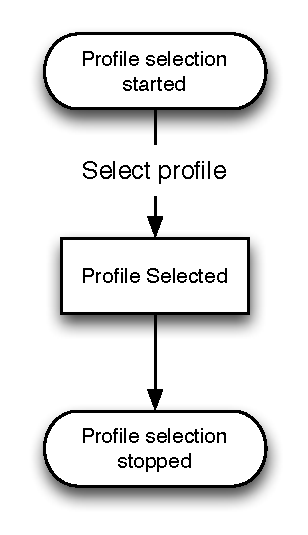
\includegraphics[width=0.5\textwidth]{gfx/profileselect_design.pdf}
	\caption{Features of the Profile selection feature}
	\label{fig:profileselection_design}
\end{figure}

The initial state of this feature is to choose which profile the previous selected should be launched as. This is done by clicking on the chosen profile. If the chosen profile is not visible on the screen, it can be needed to scroll through the profiles in order to find it. When the chosen profile is clicked the profile selection process is over.